\subsection{Proprietà sviluppi taylor}
\subsubsection{Somma}
Dati due due sviluppi di taylor
\[
	f\left( x \right) = P_1\left( x \right)  + o\left( x^{n} \right) \quad g\left( x \right) = P_2\left( x \right)  + o\left( x^{n} \right)
\]
allora lo sviluppo della somma di $f\left( x \right) $ e $g\left( x \right) $ è
\[
	P_1\left( x \right)  + P_2\left( x \right) + o\left( x^{n} \right)
\]
\subsubsection{Prodotto}
Dati due due sviluppi di taylor
\[
	f\left( x \right) = P_1\left( x \right)  + o\left( x^{n} \right) \quad g\left( x \right) = P_2\left( x \right)  + o\left( x^{n} \right)
\]
allora lo sviluppo del prodotto di $f\left( x \right) $ e $g\left( x \right) $ è
\[
	P_1\left( x \right)  \cdot P_2\left( x \right) + o\left( x^{n} \right)
\]
NB: quando si moltiplica $P_1$ con $P_2$ tutti i termini di grado $ >n$ vengono inglobati all'interno di $o\left( x^{n} \right) $, non serve quindi calcolarli
\subsection{Composta}
Dati due due sviluppi di taylor
\[
	f\left( x \right) = P_1\left( x \right)  + o\left( x^{n} \right) \quad g\left( x \right) = P_2\left( x \right)  + o\left( x^{n} \right)
\]
allora lo sviluppo della funzione composta $f\left( g\left( x \right)  \right) $
\[
	P_1\left( x \right)  \cdot P_2\left( x \right) + o\left( x^{n} \right)
\]
\subsubsection{Esempi di sviluppi}
\textbf{Esempio 1}
\[
	\cos x + 2 \sin x
\]
\begin{align*}
	\cos x            & =  1-\frac{x^2}{2}+\frac{x^{4}}{24} + o\left( x^{4} \right)                           \\
	\sin x            & =  x - \frac{x^3}{6} + o \left( x^{4} \right)                                         \\
	\cos x + 2 \sin x & =  1 - \frac{x^2}{2} + \frac{x^{4}}{24} + 2x - \frac{x^3}{3} + o \left( x^{4} \right) \\
	                  & = 1 + 2x - \frac{x^2}{2} - \frac{x^3}{3} + \frac{x^{4}}{ 24} + o\left( x^{4} \right)
\end{align*}
\textbf{Esempio 2}
\[
	\arctan x + \sinh x
\]
\begin{align*}
	\arctan x \cdot \sinh x & = \left( x- \frac{x^3}{2} + \frac{x^{5}}{5} + o\left( x^{5} \right)  \right) \left( x + \frac{x^3}{6} + \frac{x^{5}}{120} + o \left( x^{5} \right)  \right) \\
	                        & = x^2 - \frac{1}{6}x^{4} + o\left( x^{5} \right)
\end{align*}
NB: se venisse chiesto (come è purtroppo già accaduto) di dire quanto vale, ad esempio $f^{\left( 4 \right) }\left( 0 \right) $ non è conveniente derivare, ci si incasina. Bisogna invece
\begin{itemize}
	\item Calcolare lo sviluppo di Taylor con $n=4$
	\item Realizzare che il coefficiente del termine di grado 4 è uguale a $\frac{f^{\left( 4 \right) }\left( 0 \right)}{4!} $
\end{itemize}

\section{Convessità}
\begin{definizione}{Convessità/concavità sottoinsiemi}
	Un sottoinsieme $ A \subseteq \R$ si dice \underline{convesso }se per ogni coppia di punti $x,y \in  A$ allora
	\[
		\left[ x,y \right] \subseteq A
	\]

\end{definizione}
NB: ciò accade per 3 tipi di insieme:
\begin{itemize}
	\item $A \cong \R$
	\item Ogni semiretta: $\left( -\infty, a \right) \quad (-\infty, a ]  \quad [a, + \infty) \quad \left( a,+ \infty \right) $
	\item Gli intervalli: $\left( a,b \right) \quad [a,b) \quad (a, b] \quad \left[ a,b \right] $
\end{itemize}

\begin{definizione}{Convessità geometrica}
	Sia $A \subseteq  \R$ convesso. Una funzione $f : A \to \R$ si dice \underline{ convessa }se per ogni coppia di punto $P, Q$ nel grafico di $f$ tutto il segmento $PQ$ sta sopra il grafico

\end{definizione}

\begin{definizione}{Convessità algebrica}
	Sia $A \subseteq \R$. Una funzione $f: A \to \R$ si dice convesso se $ \forall a,b \in  A \quad \forall \lambda \in \left[ 0,1 \right] $
	\[
		f\left( \lambda  a + \left( 1-\lambda  \right) b \right) \le \lambda f\left( a \right)  + \left( 1-\lambda  \right) f\left( b \right)
	\]

\end{definizione}
Interpretazione geometrica:
\begin{itemize}
	\item la quantità $\lambda a + \left( 1- \lambda  \right) b$ con $ \lambda  \in  \left[ 0,1 \right] $ posso esprimere ogni punto compreso fra  $a$ e $b$ :
	      \begin{itemize}
		      \item $\lambda  = \frac{1}{2} \quad \rightarrow \quad \frac{a+b}{2}$
		      \item $\lambda  = 1 \quad \rightarrow a$
		      \item $\lambda  = 0 \quad \rightarrow b$
	      \end{itemize}
	\item
	\item Allo stesso modo la quantià $\lambda f\left( a \right)  + \left( 1-\lambda  \right) f\left( b \right)$ esprime un punto compreso fra $f\left( a \right) $ e $f\left( b \right) $
	\item Per ogni valore di $\lambda $ ottengo a sinistra $f\left( c \right) $ mentre a destra ottengo $g\left( c \right) $ dove g è la retta passante per $a\left( f\left( a \right)  \right) , \left( b,f\left( b \right)  \right)  $ con $c \in  \left[ a,b \right] $
\end{itemize}
\subsection{Convessità e derivata}
Sia $ A \subseteq  \R$ convesso e sia $ f: A \to \R$. Sappiamo che $f''\left( x \right) $ esiste $ \forall x \in  A$. Posso affermare con certezza che:
\begin{itemize}
	\item se $f''\left( x \right)  > 0 \forall x \in  A \rightarrow f$ è strettamente crescente
	\item se $f''\left( x \right)  \ge 0 \forall x \in  A \rightarrow f$ è debolmente crescente
	\item $f$ è debolmente crescente $ \Rightarrow f''\left( x \right) \ge 0 \forall  x \in A$
\end{itemize}
NB: è falso affermare che
\begin{itemize}
	\item se $f$ è strettamente crescente $ \Rightarrow f''\left( x \right) > 0 $
\end{itemize}
basti pensare alla funzione $x^4$.Pur essento \underline{strettamente concava} la sua derivata si annulla in 0
\section{Teoria di integrazione}
\subsection{Come si indicano}
\[
	\int_{a}^{b} f\left( x \right)  \; dx
\]
\begin{itemize}
	\item $\left[ a,b \right] $ zona di integrazione, cioè l'insieme in cui integriamo
	\item $f: \left[ a,b \right] $ la funzione che si integra (integranda)
	\item $dx$ simbolo che indica la variabile di integrazione
	\item la funzione $f$ è liminata in $\left[ a,b \right] $
\end{itemize}
\subsection{Significato geometrico}
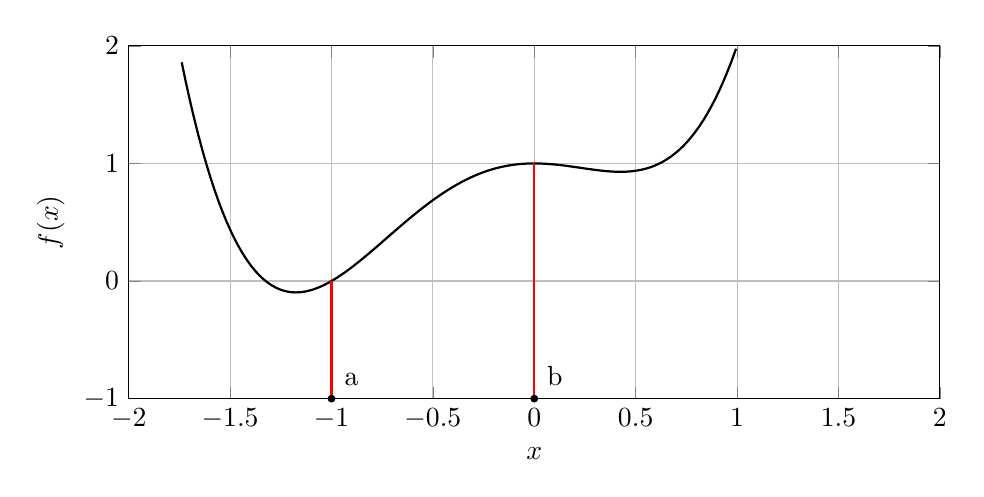
\begin{tikzpicture}
	\begin{axis}[
			xmin=-2, xmax=2,
			ymin=-1,ymax=2,
			restrict y to domain = -1:2, domain=-2:2, width=0.98\textwidth, height=0.5\textwidth, grid=major, samples=200,  ylabel=$f(x)$, xlabel=$x$]
		\addplot[black, thick] {x^3 - x^2+ x^4+1};
		\draw [red, thick] (-1,0) to (-1,-1);
		\draw [red, thick] (0,1) to (0,-1);
		\coordinate (p1) at (0,-1);
		\coordinate (p2) at (-1,-1);
	\end{axis}
	\node [label=45: a , fill=black, circle, inner sep = 1pt] at (p2) {};
	\node [label=45: b , fill=black, circle, inner sep = 1pt] at (p1) {};
\end{tikzpicture}
Come in figura, l'integrale rappresenta l'area sottesa al grafico della funzione fra $ a $ e $ b $. In questo caso è:
\[
	\int_{a}^{b} f\left( x \right)  \; dx
\]
\subsection{Definizione formale}
\begin{itemize}
	\item Caso banale \rarr funzioni costanti
	\item Caso semi-banale \rarr funzioni a gradino
	\item Caso generale
\end{itemize}
\textbf{Caso 1:}
\[
	f\left( x \right)  = \lambda \in  \R \quad \quad \forall x \in  \left[ a,b \right]
\]
In questo caso l'area è chiaramente l'area del rettangolo contenuto sotto $f\left( x \right) $
\[
	\int_{a}^{b} f\left( x \right)  \; dx = \left( b-a \right) \lambda
\]
\textbf{Caso 2:}
\[
	\text{ La funzione è costante su determinati sotto intervalli di } \left[ a,b \right]
\]
L'area in questo caso è chiaramente la somma dell'area di ogni rettangolo creato da ogni sotto intervallo costante di $ f\left( x \right) $
\[
	\int_{a}^{b} f\left( x \right)  \; dx = \sum_{k=1}^{n} \left( b-a \right) \lambda_k
\]
\textbf{Caso 3}
\[
	\text{ La funzione non è ne costante ne a scalini ma \underline{limitata} }
\]
In questo caso procedo nel seguente modo:
\begin{itemize}
	\item Provo ad approssimare l'area del grafico sotteso alla funzione tramite funzione a scalini
	\item Considero rispettivamente la funzione a gradini che stima l'area \underline{dal sopra} e \underline{dal sotto}
	\item Sia $ f : \left[ a,b \right] \to \R$ limitata. Si dice \underline{integrale superiore di $f$ in $\left[ a,b \right] $}
	      \[
		      I^{+}\left( f, \left[ a,b \right]  \right) = inf \left\{ \int_{a}^{b} p\left( x \right)   \; dx : p:\left[ a,b \right] \to \R \text{ f. a gradino t.c. } p\left( x \right) \ge f\left( x \right)  \right\}
	      \]
	      Analogamente si definisce l'integrale inferiore:
	      \[
		      I^{-}\left( f, \left[ a,b \right]  \right) = sup \left\{ \int_{a}^{b} p\left( x \right)   \; dx : p:\left[ a,b \right] \to \R \text{ f. a gradino t.c. } p\left( x \right) \le f\left( x \right)  \right\}
	      \]
	      Fatto generale molto intuitivo:
	      \[
		      I^{+}\left( f, \left[ a,b \right]  \right) \ge I^{-} \left( f, \left[ a,b \right]  \right)
	      \]
	\item Se accade che $ I^{+}\left( f, \left[ a,b \right]  \right) = I^{-} \left( f, \left[ a,b \right]  \right)  $ allora si dice che $f:  \left[ a,b \right] \to \R$ è \underline{integrabile} su $ \left[ a,b \right] $ e il valore ottenuto si indica con in simbolo
	      \[
		      \int_{a}^{b} f\left( x \right)  \; dx
	      \]
\end{itemize}
\subsection{Teoremi integrabilità}
\begin{teorema}{Integritabilità funzione}
	I seguenti tipi di funzione sono integrabili:
	\begin{itemize}
		\item Tutte le funzioni \underline{monotone} (anche non continue)
		\item Tutte le funzioni \underline{continue}
		\item Tutte le funzione che hanno un numero finito di punti di discontinuità nei quali i limini destro e sinistro esistono
	\end{itemize}
\end{teorema}

Dimostrazione per funzioni monotone:
\begin{itemize}
	\item Se per un dato $\epsilon < 0 $ trovo una somma di Riemann superiore e una inferiore la cui differenza è $ < \epsilon $ sono a cavallo
	\item Divido il grafico di  $f\left( x \right) $ in $n$ parti uguali e creo somma di Riemann dall'alto:
	      \begin{itemize}
		      \item La somma di Riemann superiore prenderà come altezza di ogni intervallo il valore della funzione di destra
		      \item La somma di Riemann inferiore prenderà come altezza di ogni intervallo il valore della funzione di sinistra
	      \end{itemize}
\end{itemize}

\begin{center}
	\input{Images/Riemann.pdf_tex}
\end{center}

\subsection{Proprietà integrali}
\[
	\begin{lgathered}
		\int_{a}^{b} \left( f\left( x \right) + g\left( x \right)  \right)  \; dx =  \int_{a}^{b} f\left( x \right)  \; dx + \int_{a}^{b} g\left( x \right)  \; dx\\
		\int_{a}^{b} \lambda f\left( x \right)  \; dx =  \lambda \int_{a }^{b} f\left( x \right)  \; dx\\
		\left|\int_{a}^{b} f\left( x \right)  \; dx\right| \le \int_{a}^{b} \left|f\left( x \right) \right|  \; dx\\
		\int_{a}^{b} f\left( x \right)  \; dx = \int_{a}^{c} f\left( x \right)  \; dx + \int_{c}^{b} f\left( x \right)  \; dx \text{ con } c \in  \left[ a,b \right] \\
		\text{ Se } f\left( x \right)  \ge g\left( x \right) \forall x \in  \left[ a,b \right]  \text{ allora }  \int_{a}^{b} f\left( x \right)  \; dx \ge \int_{a}^{b} g\left( x \right)  \; dx\\
	\end{lgathered}
\]
\section{Calcolo di integrali e integrazione impropria}
\subsection{Teoremi e definizioni}
\begin{definizione}{Primitiva di una funzione}
	Sia $ f: \left[ a,b \right]  \to \R $ continua. Si dice \underline{primitiva} di $f$ una qualunque funzione $ F: \left[ a,b \right] \to \R$ tale che $F$ è derivabile in $ \left[ a,b \right] $ e vale
	\[
		F'\left( x \right) = f\left( x \right) \quad  \forall x \in  \left[ a,b \right]
	\]

\end{definizione}

\begin{definizione}{Funzione integrale}
	Sia $ f: \left[ a,b \right] \to \R$ continua. Si dife funzione integrale la funzione:
	\[
		\Phi \left( x \right)  = \int_{a}^{x} f\left( t \right)  \; dt
	\]

\end{definizione}
NB: la funzione integrale gode delle seguenti proprietà:
\[
	\begin{lgathered}
		\int_{a}^{b} f\left( x \right)  \; dx = \Phi \left( b \right) = \left[ \Phi \left( x \right)  \right] _a ^b\\
		\int_{c}^{d} f\left( x \right)  \; dx = \Phi \left( d \right) - \Phi \left( c \right)
	\end{lgathered}
\]
\begin{teorema}{Teorema della media integrale}
	Sia $ f: \left[ a,b \right] \to \R $ continua. Allora esiste almeno un punto $c \in  \left[ a,b \right] $ tale che:
	\[
		\int_{a}^{b} f\left( x \right)  \; dx = f\left( c \right) \left( b-a \right)
	\]
\end{teorema}

\begin{teorema}{Teorema fondamentale del calcolo integrale}
	Sia $ f: \left[ a,b \right] \to \R $  continua. Sia $  \Phi  $ la sua funzione integrale. Allora
	\[
		\Phi ' \left( x \right)  = f\left( x \right) \quad \forall x \in  \left[ a,b \right]
	\]
	ossia $ \Phi  $ è primitiva di $ f $
\end{teorema}

Dimostrazione:
\begin{itemize}
	\item Calcolo il rapporto incrementale di $  \Phi  $ per $ h > 0  $
	      \[
		      \frac{\Phi \left( x+h \right) - \Phi \left( x \right) }{h}= \frac{1}{h}\left[ \int_{x}^{x+h} f\left( t \right) dt \; dt - \int_{a}^{x} f\left( t \right)  \; dt \right]
	      \]
	\item Noto che per addizione di integrali posso riscrivere il membro di destra come
	      \[
		      \frac{1}{h} \int_{x}^{x+h} f(t) \; dt
	      \]
	\item Per il teorema dei valori intermedi so che esiste un punto $ \in \left[ x, x+h \right]  $ tale che $  f\left( c \right) = \int_{x}^{x+h} f\left( x \right)  \; dx$ quindi:
	      \[
		      \frac{1}{h} \cdot h \cdot f\left( c \right)
	      \]
	\item Noto che se $ h \to 0 $ allora $  c \to x $, per cui $ f\left( c \right) \to f\left( x \right)  $. Questa affermazione posso farla in quanto $  f\left( x \right)  $ è \underline{continua}
	\item Se applico il limite per $ h \to 0 $ al rapporto incrementale ottengo che
	      \[
		      \Phi '\left( x \right) = \lim_{h \to 0} \frac{\Phi \left( x+h \right) -\Phi \left( x \right) }{h} = \lim_{h \to 0} f\left( c \right) = f\left( x \right)
	      \]
	      ho quindi dimostrato che $ \Phi  $ è derivabile e che $ \Phi '\left( x \right)  = f\left( x \right) $ ossia che $ \Phi  $ è una primitiva di $ f $
\end{itemize}
\subsection{Integrazione di funzioni razionali}
Una funzione razionale è una funzione del tipo
\[
	\frac{P\left( x \right) }{q\left( x \right) }
\]
Per integrare una cosa di questo tipo devo seguire 4 passaggi:
\begin{itemize}
	\item Divisione
	\item Fattorizzazione del denominatore
	\item Risolvere sistema lineare
	\item Integrazione
\end{itemize}
\subsubsection*{Divisione} Se il grado di $ P $ è $ < $ del grado di $ Q $ si passa al punto 2, altrimenti divido $ P\left( x \right)  $ per $  Q\left( x \right)  $ ottenendo:
\[
	\frac{P\left( x \right) }{Q\left( x \right) }= A\left( x \right) + \frac{R\left( x \right) }{P\left( x \right) }
\]
nota che avendo diviso, la funzione $ \frac{R\left( x \right)}{P\left( x \right) }  $ ha il grado del numeratore $ < $ del grado del denominatore
\vskip3mm
\textbf{Fattorizzazione:} Scomporre il numeratore in prodotto di polinomi di primo e secondo grado con i termini di secondo grado che non sono ulteriormente scomponibili. Esempio bello:
\[
	x^{4} + 1 = x^{4} + 1 + 2x^2 - 2x^2= \left( x^2 + 1 \right)^{2}- \left( \sqrt{2} x \right) ^2 = \left( x^2 + 1 + \sqrt{2} x \right) \left( x^2 + 1 - \sqrt{2} x \right)
\]
\subsubsection*{Fattorizzazione e sistema lineare}
L'obbiettivo è riscrivere la funzione razionale come somma di funzioni razionali. In generale posso avere i seguenti casi:
\begin{itemize}
	\item Al denominatore ho solo termini di grado 1. La somma sarà del tipo
	      \[
		      \frac{A}{P_1\left( x \right) }+ \frac{B}{P_2\left( x \right) }
	      \]
	\item Al denominatore ho dei termini di grado 2 non scomponibili. In questo caso, al di sopra di questi termini dovro avere un polinomio generico di grado 1:
	      \[
		      \frac{A}{P_1\left( x \right) }  + \frac{Bx + C}{P_2\left( x \right) }
	      \]
	\item Se ho fattori con molteplicità $ >1 $ devo seguire un metodo particolare spiegato dopo. In generale, ottengo qualcosa del tipo:
	      \[
		      \frac{A}{P_1\left( x \right) }+ \frac{Bx + C}{P_2\left( x \right) } + \frac{d}{dx}\left[ \frac{Fx^{n-1}\ldots  + Mx + N}{\left( P_1\left( x \right)  \right) ^{2}\left( P_2\left( x \right)  \right) ^{3}} \right]
	      \]
\end{itemize}
\hr
\subsubsection*{Esempio caso 1}
\[
	\frac{P\left( x \right) }{Q\left( x \right) }= \frac{x}{x^2-1}= \frac{x}{\left( x-1 \right) \left( x+1 \right) }= \frac{A}{x-1}+ \frac{B}{x+1}
\]
Devo cercare $ A $ e $ B $ in modo tale che venga soddisfatta l'uguaglianza fra i numeratori dei polinomi:
\[
	x=A\left( x+1 \right) +B\left( x-1 \right)
\]
Svolgo i conti a destra e raccolgo:
\[
	A\left( x+1 \right) +B\left( x-1 \right)= Ax + A + Bx - B = \left( A+B \right) x + A - B
\]
quindi ottengo il seguente sistema lineare eguagliando i coefficienti:
\[
	\begin{cases}
		A+B = 1 \\
		A-B = 0
	\end{cases}
	\rightarrow A = \frac{1}{2} \quad B = \frac{1}{2}
\]
\hr
\subsubsection*{Esempio caso 2}
Se al denominatore ho fattori di grado $ \neq 1$, dovrò trovare il valore di 3 costanti $ A, B, C $. Es:
\[
	\frac{2x^2 + 3}{x^3 - 1}= \frac{A}{x-1} + \frac{Bx + C}{x^2 + x +1}
\]
eseguendo i conti e raccogliendo:
\[
	\frac{\left( A + B \right) x^2 + \left( A- B + C \right) x + A - C}{\left( x-1 \right) \left( x^2 + x+1 \right) }
\]
e ottengo il sistema lineare a 3 incognite:
\[
	\begin{cases}
		A + B = 2    \\
		A - B + C =0 \\
		A - C = 3
	\end{cases}
	\rightarrow A= \frac{5}{3} \quad B = \frac{1}{3} \quad C = - \frac{4}{3}
\]
Quindi, in generale, dove al denominatore ho un polinomio di grado 1 sopra avrò una costante, mentre se al denominatore ho un polinomio di grado 2, al numeratore ho un polinomio generico di grado 1:
\[
	\frac{x^3 + 5}{\left( 2x + 1 \right) \left( x-3 \right) \left( x-8 \right) \left( x^2+1 \right) \left( x^2 + x +1 \right) }
\]
\[
	\frac{A}{2x+1} + \frac{B}{x-1} + \frac{C}{x-8} + \frac{Dx + E}{x^2+1}+\frac{Fx + G}{x^2 + x +1}
\]
quindi ottengo un sistema in tante incognite quanto è il \underline{grado del denominatore}
\hr
\subsubsection*{Esempio caso 3}
Se i fattori al denominatore hanno molteplicità $ > 1$ procedo nel seguente modo:
\begin{multline*}
	\frac{P\left( x \right) }{\left( x+1 \right) ^{4} \left( x+5 \right) ^2\left( x+7 \right) \left( x^2 +1 \right) ^3} =\frac{A}{x+1} + \frac{B}{x+5} + \frac{C}{x+7}+ \frac{Dx + E}{x^2+1} \\ + \frac{d}{dx}\left[ \frac{F x ^{7 }+ G x ^{6} + H x^{5}+ J x^{4}+ K x^3 + L x^2 + Mx + N}{\left( x+1 \right) ^3 \left( x+5 \right) \left( x^2 + 1 \right) ^2} \right]
\end{multline*}
Ossia:
\begin{itemize}
	\item Scrivo fattorizzazione del denominatore e la scrivo come somma, \underline{ignorando la molteplicità} di ogni termine (occhio però a non trascurare il fatto che al numeratore del termini di secondo grado andrà un polinomio di primo)
	\item A questo aggiungo la derivata di un polinomio in cui ho:
	      \begin{itemize}
		      \item \underline{Al denominatore} il prodotto dei polinomi che avevo originariamente al denominatore \underline{abbassati di un grado}
		      \item \underline{Al numeratore} la somma di $ n-1 $ polinomi generici di grado $ 0,\ldots, n-1 $ dove $ n $ è il grado del denominatore
	      \end{itemize}
\end{itemize}
\subsubsection*{Integrazione}
Svolti i passaggi spiegati precedentemente posso ritrovarmi 3 tipi di funzioni da integrare:
\begin{itemize}
	\item Funzioni del tipo $ \displaystyle \frac{k}{ax + c} $, integrate, diventano semplici logaritmi
	\item Funzioni del tipo $ \displaystyle \frac{P_1\left( x \right) }{P_2\left( x \right) } $ dove $ p_1 $ è di grado 1 e $ P_2 $ è grado 2 \underline{non scomponibile}, integrate, diventano arcotangenti. Devo usare completamento del quadrato al denominatore
\end{itemize}

\subsection{Trucchetti integrazione}
\subsubsection*{Integrazione radici di polinomi di secondo grado}
\[
	\boxed{\int \sqrt{1-x^2}}
\]
Metodo trigonometrico
\begin{itemize}
	\item Sostituzione $ x=\sin \left( y \right)  $
	\item Uso formule trigonometriche tenendo conto che $ 1-\sin ^2 \left( y \right) = \cos ^2 y $
\end{itemize}
Metodo della sostituzione
\begin{itemize}
	\item Scrivo come somma per differenza
	\item Sostuisco l'intera radice con uno dei due termini $ =y $ e l'altro rimane invariato. Es $ \sqrt{x^2 -1} =\sqrt{\left( x+1 \right) \left( x-1 \right) } = y\left( x-1 \right)  $
	      i
\end{itemize}
Più in generale, se ho un polinomio con due radici reali $ \lambda, \rho   $, allora posso applicare la sostituzione:
\[
	\sqrt{ \text{ polinomio }} = y\left( x- \lambda  \right) \text{ oppure } \sqrt{ \text{ polinomio }} =y \left( x-\rho \right)
\]

\hr
\[
	\boxed{\int \sqrt{x^2 + 1}}
\]
Metodo trigonometrico
\begin{itemize}
	\item Sostituzione $ x = \sinh y $
	\item Uso formule trigonometriche tenendo conto che $ \sinh^2 + 1 = \cosh ^2 $
	\item Posso integrare $ \sinh ^2 y $ in 3 modi:
	      \begin{itemize}
		      \item Scrivendo esplicitamente il $ \sinh $ tramite esponenziale
		      \item Scrivendo la formula di duplicazione $ \sinh \left( 2x \right)  $
		      \item Utilizzo la formula per parti in maniera \underline{ciclica}
	      \end{itemize}

\end{itemize}
Metodo della sostituzione
\begin{itemize}
	\item Sostituzione $ \sqrt{x^2 + 1} = y + x $
	\item Noto che così facendo $ x^2 $ sparisce e dunque posso ricavare $ x $ in funzione di $ y $
\end{itemize}
Nota che se il coefficiente di $ x^2 $ non è 1, la sostituzione da fare è diversa, ad esempio
\[
	\int \sqrt{ax^2 + bx + c} \; dx \rightarrow \sqrt{ax^2 + bx + c} = \sqrt{a} x + y
\]
in modo tale che eseguendo il quadrato si elimini il termine di secondo grado
\subsubsection*{Sostituzioni parametriche}
Possa "convertire" un seno o un cosno in un polinomio tramite le formule parametriche:
\[
	\sin x = \frac{2y}{y^2 + 1} \quad \cos  x = \frac{1- y^2}{y^2 + 1}
\]
ponendo
\[
	y= \tan  \frac{x}{2}
\]
Inserendo $ \tan \frac{x}{2} $ all'interno delle due formule parametriche si può verificare che l'uguaglianza è verivicata. L'integrale di $ \frac{1}{\sin \left( x \right) } $ può essere risolto in due modi:
\begin{itemize}
	\item Formule parametriche
	\item Moltiplicando e dividendo per seno, ricordando che $ \sin ^2 x  = 1- \cos ^2 x$ e ponendo $ y=\cos x $
\end{itemize}
NB: i casi in cui le sostituzioni parametriche semplificano il tutto sono molto rari, quindi generalmente queste si usano come \underline{ultima spiaggia}
\hr
\[
	\boxed{\frac{1}{ \cos ^3 \left( x \right) \sin ^3 \left( x \right) }}
\]
\begin{itemize}
	\item Sostituzioni parametriche (troopo complicati i conti)
	\item Uso formula di duplicazione: $ \sin x \cos x = \frac{1}{2} \sin  \left( 2x \right)  $.
	      \begin{itemize}
		      \item	Se la potenza ottenuta è dispari moltiplico e diviso per $ \sin \left( 2x \right)  $, ottenento potenza pari al denominatore
		      \item La riscrivo usando che $ \sin ^2 \left( 2x \right) = 1- \cos ^2\left( 2x \right)  $
		      \item	Integro funzione razionale con molteplicità
	      \end{itemize}
	\item Scrivo $ 1=\sin ^2 \left( x \right)  + \cos  ^2 \left( x \right)  $
\end{itemize}
\subsection{Integrali imporpri}
Ho due tipi di integrali impropri:
\begin{itemize}
	\item Integrali calcolati su intervallo non limitato:
	      \[
		      \int_{a}^{\infty} f\left( x \right)  \; dx \quad \int_{-\infty}^{a} f\left( x \right)  \; dx
	      \]
	\item Integrali calcolati su intervallo limitato $ \left[ a,b \right]  $in cui \underline{la funzione} non è limitata in $ x=a $ o $ x=b $
\end{itemize}
Se l'integrale non ricade in nessuna di queste due categorie, posso ricondurlo ad una di esse spezzandolo in più parti.
\subsubsection*{Esempio 1}
\begin{center}
	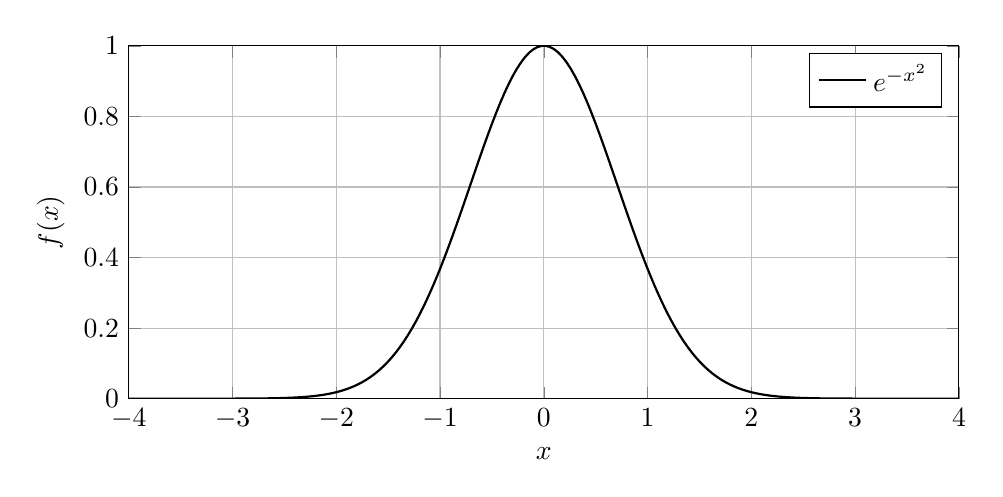
\begin{tikzpicture}
		\begin{axis}[
				xmin=-4, xmax=4,
				ymin=0,ymax=1,
				restrict y to domain = 0:3, domain=-4:4, width=\textwidth, height=0.5\textwidth, grid=major, samples=200,  ylabel=$f(x)$, xlabel=$x$, legend entries={$ e^{-x^2} $}]
			\addplot[black, thick] {e^(-x^2)};
		\end{axis}
	\end{tikzpicture}
\end{center}
Per calcolare l'integrale seguente posso spezzarlo in due parti
\[
	\int_{-\infty}^{\infty} e^{-x^2} \; dx= \int_{-\infty}^{a} e^{-x^2} \; dx + \int_{a}^{\infty} e^{-x^2} \; dx
\]
in questo caso $ a $ deve essere necessariamente 0 in quanto in 0 la funzione \underline{non} è definita
\subsubsection*{Esempio 2}
\begin{center}
	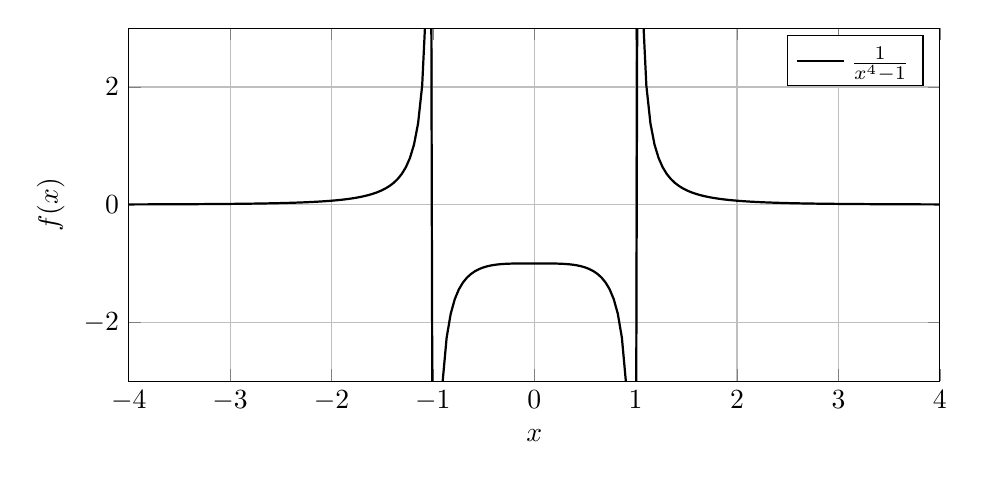
\begin{tikzpicture}
		\begin{axis}[
				xmin=-4, xmax=4,
				ymin=-3,ymax=3,
				restrict y to domain = -30:30, domain=-4:4, width=0.98\textwidth, height=0.5\textwidth, grid=major, samples=200,  ylabel=$f(x)$, xlabel=$x$, legend entries={$\frac{1}{x^{4}-1} $}]
			\addplot[black, thick] {1/(x^4-1)};
		\end{axis}
	\end{tikzpicture}
\end{center}
Per calcolare l'integrale
\[
	\int_{-\infty}^{\infty} \frac{1}{x^{4}-1} \; dx
\]
devo spezzarlo nei punti $ \left( -\infty, -3 \right) , \left( -3, -1 \right) , \left( -1, 0 \right) , \left( 0,1 \right) , \left( 1,3 \right) , \left( 3, +\infty \right)  $:
\[
	\int_{-\infty}^{\infty} \frac{1}{x^{4}-1} \; dx = \int_{-\infty}^{-3}  \; dx + \int_{-3}^{1}  \; dx + \int_{-1}^{0}  \; dx + \int_{0}^{1}  \; dx + \int_{1}^{3}  \; dx + \int_{3 }^{+\infty}  \; dx
\]
\subsubsection*{Esempio 3}
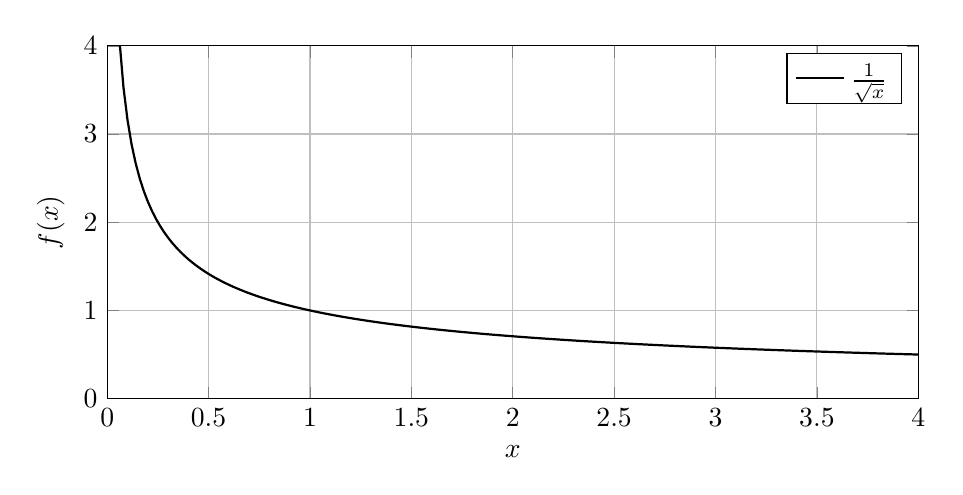
\begin{tikzpicture}
	\begin{axis}[
			xmin=0, xmax=4,
			ymin=0,ymax=4,
			restrict y to domain = 0:30, domain=0:4, width=0.98\textwidth, height=0.5\textwidth, grid=major, samples=200,  ylabel=$f(x)$, xlabel=$x$, legend entries={$ \frac{1}{\sqrt{x} }$}]
		\addplot[black, thick] {1/(sqrt(x))};
	\end{axis}
\end{tikzpicture}
\[
	\int_{0}^{5} \frac{1}{\sqrt{x} } \; dx= \lim_{a \to 0} \int_{a}^{5} \frac{1}{\sqrt{x} } \; dx
\]
\subsubsection*{Esempio 4}
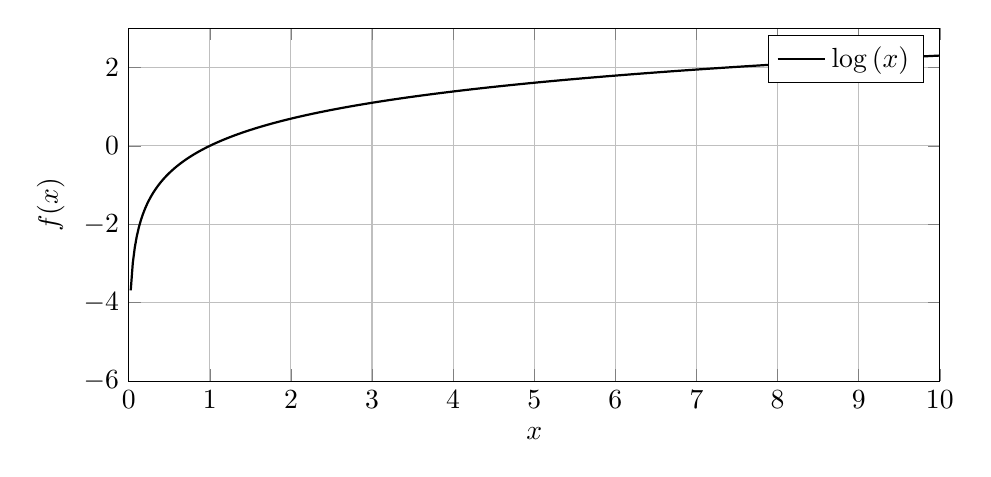
\begin{tikzpicture}
	\begin{axis}[
			xmin=0, xmax=10,
			ymin=-6,ymax=3,
			restrict y to domain = -400:30, domain=0:10, width=0.98\textwidth, height=0.5\textwidth, grid=major, samples=400,  ylabel=$f(x)$, xlabel=$x$, legend entries={$ \log \left( x \right) $}]
		\addplot[black, thick] {ln(x)};
	\end{axis}
\end{tikzpicture}
\[
	\int_{0}^{5} \log \left( x \right)  \; dx = \lim_{a \to 0} \int_{a}^{5} \log \left( x \right)  \; dx
\]
NB: un integrale improprio, essendo per definizione un limite, può non esistere. Ad esempio $ \int_{0}^{+\infty} \sin \left( x \right)  \; dx $ \underline{non esiste} in quanto oscilla infinitamente
\subsection{Teorema del confronto}
Spesso, vogliamo determinare se un integrale improprio corverga o meno, ma non sappiamo calcolarne una primitiva. In questi casi torna utile il \underline{teorema del comfronto}. L'idea è la seguente
\begin{itemize}
	\item Determino se funzioni campione delle quali so calcolare la primitiva convergono o meno
	\item Utilizzo queste funzioni, confrontandole con quella di cui devo determinare la convergenza
\end{itemize}
In particolare, le funzione "campione" che useremo saranno funzioni del tipo
\[
	\frac{1}{x^{\alpha }}
\]
in particolare queste funzioni vengono dette gli \underline{infiniti campione}.
\[
	\int_{1}^{+\infty} \frac{1}{x^{\alpha }} \; dx
\]
\begin{itemize}
	\item Converge se $ \alpha  >1 $
	\item Diverge se $ \alpha \le 1 $
\end{itemize}
Se invece considero l'integrale sull'intervallo $ \left( 0,1 \right)  $ ho che:
\[
	\int_{0}^{1} \frac{1}{x^{\alpha }} \; dx
\]
\begin{itemize}
	\item Converge se $ \alpha < 1 $
	\item Diverge se $ \alpha  \ge 1 $
\end{itemize}
Ciò risulta chiaro se osserviami i grafici delle funzioni
\begin{center}
	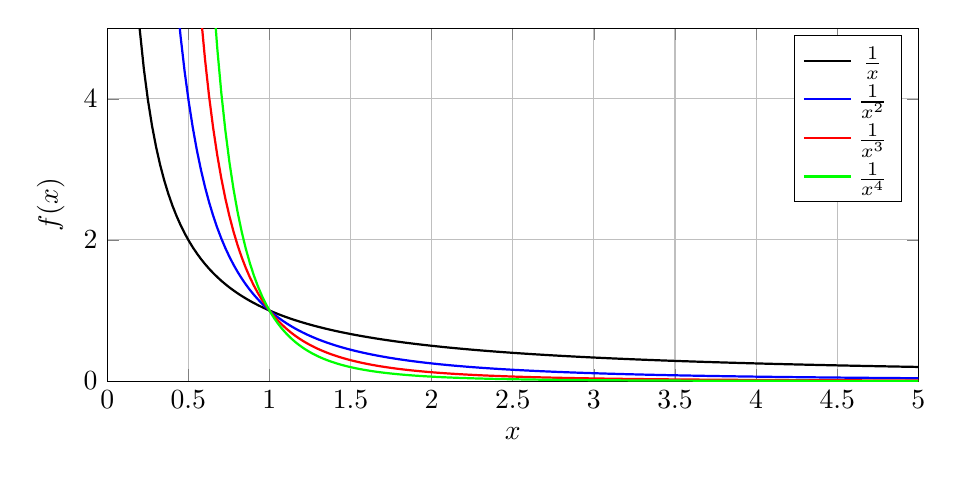
\begin{tikzpicture}
		\begin{axis}[
				xmin=0, xmax=5,
				ymin=0,ymax=5,
				restrict y to domain = 0:500, domain=0:5, width=0.98\textwidth, height=0.5\textwidth, grid=major, samples=200,  ylabel=$f(x)$, xlabel=$x$, legend entries={$\frac{1}{x}$,$\frac{1}{x^{2}}$, $\frac{1}{x^3}$ , $\frac{1}{x^4}$}]
			\addplot[black, thick] {1/x};
			\addplot[blue, thick] {1/x^2};
			\addplot[red, thick] {1/x^3};
			\addplot[green, thick] {1/x^4};
		\end{axis}
	\end{tikzpicture}
\end{center}
\begin{teorema}{Criterio del confronto}
	Sia $ f\left( x \right)  $ una funzione integranda, della quale voglio determinare l'ipotetica convergenza, su intervallo limitato o non. Sia $ g\left( x \right)  $ un infinito campione del tipo $ \frac{1}{x^{\alpha }} $. Se $ 0 \le f\left( x \right) \le g\left( x \right)  $ almeno in un intorno del problema (estremi intervallo integrazione, $ +\infty, - \infty $), allora:
	\[
		\text{ se }\int_{E} g\left( x \right)  \; dx \text{ converge } \Rightarrow \int_{E} f\left( x \right) \; dx \text{ converge }
	\]
	\[
		\text{ se }\int_{E} f\left( x \right)  \; dx \text{ diverge } \Rightarrow \int_{E} g\left( x \right) \; dx \text{ diverge }
	\]

\end{teorema}

\begin{teorema}{Teorema del confronto asintotico}
	Supponiamo che $ f\left( x \right) \ge 0 $ e $ g\left( x \right) > 0 $. Allora se
	\[
		\lim_{x \to x_0} \frac{f\left( x \right) }{g\left( x \right) } \neq 0, \infty
	\]
	allora l'integrale delle due funzioni si comporta nello stesso modo (convergenza/divergenza è uguale)

\end{teorema}

Se $ \lim_{x \to x_0} \frac{f\left( x \right) }{g\left( x \right) }  = 0 $
\begin{itemize}
	\item Se $ \int_{E} g\left( x \right)  \; dx $ converge allora $ \int_E f\left( x \right)  \; dx $ converge
	\item Altrimenti non so dire nulla
\end{itemize}
Se $ \lim_{x \to x_0} \frac{f\left( x \right) }{g\left( x \right) }  = +\infty $
\begin{itemize}
	\item Se $ \int_{E} g\left( x \right)  \; dx $ diverge allora $ \int_E f\left( x \right)  \; dx $ diverge
	\item Altrimenti non so dire nulla
\end{itemize}
\subsubsection*{Assoluta integrabilità}
Questo teorema può essere utile per applicare il teorema del confronto su funzioni che non sono sempre $ \ge 0  $ o $ \le 0 $.

\begin{teorema}{Assoluta integrabilità}
	\[
		\text{ Se }\int_{E}\left|f\left( x \right) \right| \; dx \text{ converge } \Rightarrow \int_{E} f\left( x \right)  \; dx \text{ converge }
	\]
	\[
		\text{ Se } \int_{E}\left|f\left( x \right) \right| \; dx \text{ diverge } \rightarrow \text{ non posso affermare nulla }
	\]

\end{teorema}
Ad esempio:
\[
	\int_{0}^{+ \infty} \frac{\sin \left( x^2 \right) }{x^3} \; dx
\]
non posso utilizzare il teorema del confronto asistotico perchè il seno non è sempre positivo. Posso tuttavia analizzare la funzione
\[
	\int_{0}^{+ \infty} \frac{\left|\sin \left( x^2 \right) \right| }{x^3} \; dx
\]
\begin{itemize}
	\item Considero che la funzione integranda è maggiorata dalla funzione $ \frac{2}{x^3} $
	      \[
		      \frac{\left|\sin \left( x^2 \right) \right|}{x^3} \le \frac{2}{x^3}
	      \]
	\item Siccome la funzione $ \frac{2}{x^3} $ converge, allora anche $ \frac{\left|\sin \left( x^2 \right) \right|}{x^3} $ converge.
	\item  Se $ \frac{\left|\sin \left( x^2 \right) \right|}{x^3} $ converge, per il teorema della assoluta integrabilità, anche $\frac{\sin \left( x^2 \right) }{x^3} $
\end{itemize}
\subsection{Trucco dell'integrazione per parti}
Se devo decretare la convergenza/divergenza di un integrale improprio posso utilizzare il metodo dell'integrazione per parti. Consideriamo il seguente esempio:
\subsubsection*{Esempio 1}
\[
	\int_{1}^{ + \infty} \frac{\sin x}{x} \; dx
\]
non posso applicare il teorema del confronto in quanto ogni funzione $ \frac{1}{x^{\alpha }} $ con $ \alpha \ge 1 $  è definitivamente minore di $ \frac{\sin x}{x} $ e converge. Contrariamente, $ \frac{1}{x} $ è definitivamente maggiore, però diverge per $ x \to \infty $	e non posso dunque affermare nulla. Se integro per parti tuttavia:
\[
	\int \frac{\sin x}{x} \; dx = \frac{1}{x} \left( - \cos  x \right) - \int -\frac{1}{x^2}\left( -\cos x \right)
\]
applicando il limite posso decretare che l'integrale converge
\subsubsection*{Esempio 2}
\[
	\int_{0}^{+\infty} \cos \left( x^2 \right)  \; dx
\]
stranamente, questo integrale converge ad un numero reale. Non posso applicare assoluta integrabilità perchè, chiaramente, l'integrale del suo valore assoluto diverge. Provo moltiplicando e dividendo per $ x $ (in modo da ottenere la derivata della composta), per poi integrare per parti:
\[
	\int \cos \left( x^2 \right) = \int \frac{1}{x} x \cos \left( x^2 \right) = \left( -\frac{1}{x^2} \right)  \left( \frac{1}{2}\sin \left( x^2 \right) \right)  - \int  \left( -\frac{1}{x^2} \right) \frac{1}{2}\sin \left( x^2 \right)
\]
Visto che ogni membro converge, posso affermare che $ \int_{0}^{+ \infty} \cos \left( x^2 \right)  \; dx $ \underline{converge}

\section{Equazioni differenziali}
\subsection{Definizioni}
\begin{definizione}{Equazione differenziale}
	Con il termine \underline{equazione differenziale} si intende una relazione tra una \underline{funzione incognita} e le sue derivate. Posso interpretarla come una funzione di più variabili:
	\[
		F\left( t, u\left( t \right) , u'\left( t \right) ,\ldots, u^{\left( k \right) }\left( t \right)  \right)=0
	\]
	dove $ t, u\left( t \right) ,\ldots, u^{\left( k \right) }\left( t \right)  $ sono le incognite dell'equazione differenziale

\end{definizione}
La soluzione di un'equazione differenziale è un'equazione che risolve l'uguaglianza specificata
\begin{itemize}
	\item \textbf{Ordine}: l'ordine di un'equazione differenziale è uguale al massimo ordine di derivazione presente nell'equazione
	\item \textbf{Eq diff. in forma normale}: una eq. diff. si dice in forma normale se si può "isolare" la derivata di ordine massimo:
	      \[
		      u^{\left( k \right) } = \Phi \left( u^{\left( k-1 \right) },\ldots, u\left( t \right) ,t \right)
	      \]
	\item \textbf{Eq. diff. autonoma}: se la incognita $ t $ compare solo come incognita della funzione incognita (e non compe coefficiente):
	      \[
		      u^{\left( k \right) }+ u ^{\left( k-1 \right) }+\ldots+u' + u =0
	      \]
	\item \textbf{Eq. diff. a variabili separabili}: se è del \underline{primo ordine}, scritta in \underline{forma normale} e si può scrivere nella seguente forma:
	      \[
		      u'= f\left( t \right) g\left( u \right)
	      \]
	\item \textbf{Eq. diff. lineare}: se la funzione $ u $ e le sue derivate non sono presenti all'interno di funzioni. Ha forma del tipo:
	      \[
		      a_k\left( t \right) u^{\left( k \right) }+ a_{k-1}\left( t \right) u^{\left( k-1 \right) }+\ldots+ a_1\left( t \right) u'+ a_0\left( t \right) u = f\left( t \right)
	      \]
	      \begin{itemize}
		      \item $ a_0\left( t \right) , a_1\left( t \right) ,\ldots, a_k\left( t \right)  $ sono detti \underline{coefficienti}
		      \item $ f\left( t \right)  $ è detto \underline{termine noto}
		      \item Se $ f\left( t \right) =0 $ l'equazione lineare si dice \underline{omogenea}
		      \item Se $ a_0\left( t \right) , a_1\left( t \right) ,\ldots, a_k\left( t \right)  $ sono costanti l'equazione è detta a \underline{coefficienti costanti}
	      \end{itemize}
\end{itemize}

\subsubsection*{Esempio 1}
\[
	f'\left( x \right) = f\left( x \right)
\]
Quale equazione ha la derivata uguale alla equazione stessa? Esattamente l'esponenziale. Più precisamente le soluzioni di questa equazione sono \underline{infinite} ed identificate dalla seguente funzione:
\[
	k e^{x}
\]
\subsubsection*{Esempio 2}
\[
	f'\left( x \right) = - f\left( x \right) ^2
\]
una qualsiasi soluzione del seguente tipo risolve la seguente eguaglianza:
\[
	f\left( x \right) = \frac{1}{t + c}
\]
\subsubsection*{Esempio 3}
\[
	f''\left( x \right) = - f\left( x \right)
\]
noto che una soluzione è $ n\left( x \right) = \cos \left( x \right)  $. La famiglia delle soluzioni è $ n\left( x \right) = c \cos \left( t \right)  , c \in  \R$. Ancora più in generale, ogni funzione del tipo:
\[
	f\left( x \right) = c_1 \cos t\left( x \right)  + c_2 \cos \left( x \right)
\]
soddisfa l'eguaglianza. Nota che il numero di parametri che ottengo dipende dall'\underline{ordine} dell'equazione
\subsection{Problemi di Cauchy}
Negli esempi precedenti ho ottenuto le cosiddette \underline{soluzioni generali} delle equazioni differenziali. Se impongo un'ulteriore condizione sulla condizione generale ottengo il valore della costante (o delle costanti) in corrispondenza del quale è risolto il problema di Cauchy.
\subsubsection*{Esempio 1}
\[
	\begin{cases}
		u'\left( t \right) = u\left( t \right) \\
		u\left( 0 \right) = 5
	\end{cases}
\]
\begin{itemize}
	\item Condizione dell'equazione differenziale: $ ce^{t} $
	\item Condizione iniziale: $ u\left( 0 \right) = ce^{0} \rightarrow c = 5 $
\end{itemize}
Quindi la soluzione è $ 5 e ^{t} $
\subsubsection*{Esempio 2}
\[
	\begin{cases}
		u' = - u^2 \\
		u\left( 5 \right) = 7
	\end{cases}
\]
\begin{itemize}
	\item Soluzione dell'equazione differenziale: $ \frac{1}{t + c} $
	\item Condizione iniziale: $ u\left( 5 \right) = 7 $
\end{itemize}
\hr
Nota che le condizioni delle equazioni differenziali ordinarie devono essere tante quanto è l'ordine dell'equazione differenziale: ottengo infatti un sistema in cui devo trovare il valore a tutte le costanti ottenute trovando la \underline{soluzione generale}
\subsubsection*{Esempio 3}
\[
	\begin{cases}
		u'' + 3 u' = u^2 + t^2 \\
		u \left( 5 \right) = 7 \\
		u' \left( 5 \right) = 22
	\end{cases}
\]
è un problema di Cauchy.
\[
	\begin{cases}
		u'' + 3 u' = u^2 + t^2 \\
		u \left( 5 \right) = 7 \\
		u' \left( 6 \right) = 22
	\end{cases}
	\quad
	\begin{cases}
		u'' + 3 u' = u^2 + t^2 \\
		u \left( 5 \right) = 7 \\
		u'' \left( 5 \right) = 22
	\end{cases}
\]
non sono problemi di Cauchy. Più in generale
\begin{definizione}{Problema di Cauchy}
	Data un'equazione differenziale ordinaria di ornine $ n $, un problema di Cauchy associato deve:
	\begin{itemize}
		\item Specificare le \underline{condizioni iniziali} in uno stesso punto
		\item Specificare le condizioni iniziali per le derivate di ordine $ 0,1,\ldots, n-1 $
	\end{itemize}
\end{definizione}

\begin{teorema}{Teorema di esistenza}
	Consideriamo il problema di Cauchy per una equazione differenziale ordinaria. Defininiamo la funzione:
	\[
		u^{\left( k \right) }= \Phi \left( u, u',u'',\ldots,u^{\left( k-1 \right) },t \right)
	\]
	Se $ \Phi   $ è continua in ogni variabile allora esiste sempre \underline{almeno una soluzione}

\end{teorema}

la funzione $ \Phi $ è una funzione a più variabili. La sua continuità o la sua derivabilità si decreta "congelando" tutte le variabili meno che una e studiandone continuità/derivabilità
\begin{teorema}{Teorema di unicità}
	Consideriamo il problema di Cauchy per una equazione differenziale ordinaria. Defininiamo la funzione:
	\[
		u^{\left( k \right) }= \Phi \left( u, u',u'',\ldots,u^{\left( k-1 \right) },t \right)
	\]
	Se $ \Phi  $ è \underline{derivabile} in tutte le variabili, allora la soluzione è \underline{unica}

\end{teorema}
il cosiddetto "pennello" di Peano è un problema di Cauchy che presenta infinite soluzioni:
\[
	\begin{cases}
		u'= 3 \left|u\right|^{\frac{2}{3}} \\
		u\left( 0 \right) =0
	\end{cases}
\]
La funzione $ 3 \left|u\right|^{\frac{2}{3}} $ non è derivabile, quindi la soluzione \underline{non} è unica. Nota che sia $ u=0 $ che $ u=t^3 $ sono soluzioni del problema. Il problema presenta più di una soluzione
\subsection{Edo a variabili separabili}
\[
	u' = f\left( t \right) g\left( u \right)
\]
Per trovare la soluzione ci sono 3 passaggi:
\begin{itemize}
	\item Separazione
	\item Integrazione
	\item Ricavare
\end{itemize}
Esempio:
\[
	u' = t^3 u^2
\]
\begin{itemize}
	\item \underline{Separo} le variabili: metto tutto ciò che dipende da $ u $ a sinistra e tutto ciò che dipende da $ t $ a destra, usando questo trucchetto bovino:
	      \[
		      \frac{du}{dt}= t^3 u^2 \rightarrow \frac{du}{u^2}= t_3 dt
	      \]
	\item \underline{Integro} da entrambe le parti:
	      \[
		      \int \frac{du}{u^2}= \int t_3 dt \rightarrow - \frac{1}{u}= \frac{1}{4} t^{4} + c
	      \]
	\item \underline{Ricavo} $ u $ in funzione di $ t $:
	      \[
		      u\left( t \right) = \frac{- 4}{t ^{4} + c} \quad c \in  \R
	      \]
\end{itemize}
\hr

Se all'edo è associato un problema di Cauchy è necessario studiare la soluzione: il dominio della soluzione varia in base al valore di $ c $ trovato. Per questa ragione devo restringere il dominio della funzione trovata.
\textbox{Devo restringere il dominio della funzione trovata al massimo insieme di definizione che contiene il punto indicato nella condizione iniziale}
\subsection{Tempo di vita ed esempi}
\begin{definizione}{Tempo di vita}
	Trovata la funzione $ u\left( t \right)  $ soluzione di un problema di Cauchy, si dice tempo di vita l'\underline{estremo superiore} dell massimo insieme di definizione contenente il punto $ t_0 $ che esprime la condizione di essistenza.
	\begin{itemize}
		\item Se $ T=+ \infty $ si dice che $ f\left( t \right)  $ ha \underline{esistenza globale} nel futuro
		\item Se $ T < +\infty $ ci sono due casi:
		      \begin{itemize}
			      \item Se $ \lim_{x \to T^{-}} f\left( t \right) = \pm \infty  \rightarrow$ \underline{blow up}
			      \item Se non c'è blow up ma $ u\left( t \right)  $ esce dal dominio di una o più funzioni presenti nell'equazione differenziale $ \rightarrow $ \underline{break down}. In genere (ma non sempre) questo si dtraduce nella seguente condizione
			            \[
				            \lim_{x \to T^{-}} f'\left( t \right) = \pm \infty
			            \]
		      \end{itemize}
	\end{itemize}

\end{definizione}

\subsubsection*{Esempio Cauchy 1}
\[
	\begin{cases}
		u' = t^3 u^2 \\
		u\left( 0 \right) = -5
	\end{cases}
\]
L'edo ha soluzione
\[
	u\left( t \right) = \frac{-4}{t ^{4}+ c}
\]
\begin{itemize}
	\item Determino $ c $ :
	      \[
		      u\left( 0 \right) = -\frac{4}{c} \rightarrow c = \frac{4}{5}
	      \]
	      quindi il problema di Cauchy ha soluzione $ u\left( t \right)= -\frac{4}{t ^{4}+ \frac{4}{5}} $
	\item Il massimo dominio di definizione contentente $ 0 $ è $ \R $, quindi $ u\left( t \right)  $ ha \underline{esistenza globale} sia nel passato che nel futuro
\end{itemize}
\subsubsection*{Esempio Cauchy 2}
\[
	\begin{cases}
		u' = t^3 u^2 \\
		u\left( 0 \right) = 0
	\end{cases}
\]
L'edo ha soluzione
\[
	u\left( t \right) = \frac{-4}{t ^{4}+ c}
\]
\begin{itemize}
	\item Determino $ c $ :
	      \[
		      u\left( 0 \right) = -\frac{4}{c} =0
	      \]
	      Cosa faccio? Non posso risolvere l'equazione ottenuta.
\end{itemize}
In questo caso il problema di Cauchy \underline{ha una soluzione}. Tale soluzione si ottiene risolvendo la condizione iniziale:
\[
	u\left( t \right) =0
\]
in questo modo soddisfo sia la condizione iniziale $ u\left( 0 \right) =0 $ e l'equazione differenziale in quanto $ u' = t^3 u^2 $
\subsubsection*{Esempio Cauchy 3}
\[
	\begin{cases}
		u' = u^3 t^2 \\
		u\left( 0 \right) =5
	\end{cases}
\]

La soluzione dell'equazione differenzile è:
\[
	u\left( t \right) = \pm \sqrt{\frac{3}{c-2t^3}}
\]
Devo sceglere la radice positiva in quanto la condizione iniziale impone $ u\left( 0 \right) =5 $.Impongo la condizione iniziale e ottengo
\[
	\sqrt{\frac{3}{c}} \rightarrow c = \frac{3}{25}
\]
Quindi il problema di Cauchy ha soluzione
\[
	u\left( t \right) = \sqrt{\frac{3}{\frac{3}{25} - 2 t ^3}} = \sqrt{ \frac{75}{3 - 50 t^3}}
\]
Posso procedere ora studiando la soluzione:
\[
	3 - 50 t^3 > 0 \rightarrow t < \sqrt[3]{\frac{3}{50}}
\]
La funzione è quindi definita su $ \left( - \infty, \sqrt[3]{\frac{3}{50}}  \right)  $. Posso dunque affermare che il \underline{tempo di vita} della funzione è $ T= \sqrt[3]{\frac{3}{50}} $. Visto che $ \lim_{t \to \sqrt[3]{\frac{3}{50}}^{-}} u\left( t \right)   = + \infty $ la funzione ha un \underline{blow up}
\subsubsection*{Esempio Cauchy 4 parametrico}
\[
	\begin{cases}
		u' = u^3 t^2 \\
		u\left( 0 \right) = \alpha
	\end{cases}
\]
Per quali valori di $ \alpha  $ ho esistenza globale nel futuro?
\vskip3mm
Eseguo tutti i passi fatti per trovare le soluzioni del problema di Cauchy rispetto al parametro $ \alpha  $ e ottengo:
\[
	u\left( t \right) = \pm \sqrt{\frac{3}{-2t^3 + \frac{3}{\alpha ^2}}}
\]
\subsubsection*{Esempio Cauchy 4}
\[
	\begin{cases}
		u'= u \sin \left( t \right) \\
		u\left( 0 \right) = -2
	\end{cases}
\]
\begin{itemize}
	\item Separo:
	      \[
		      \frac{du}{u}= \sin \left( t \right) dt
	      \]
	\item Integro:
	      \[
		      \int \frac{du}{u}= \int \sin \left( t \right) dt \rightarrow \log \left| u\right|= - \cos t\left( t \right)  + c
	      \]
	\item Ricavo (tolgo il valore assoluto introducento $ \pm $):
	      \[
		      u\left( t \right) = \pm e^{-\cos \left( t \right)  + c}= c e ^{-\cos \left( t \right) }
	      \]
	\item Determino $ c $
	      \[
		      u\left( 0 \right) = -2 \rightarrow c = -2e
	      \]
\end{itemize}
La soluzione al problema di Cauchy è quindi:
\[
	u\left( t \right) = -2e \cdot e^{-\cos \left( t \right) }
\]
\subsubsection*{Esempio 6 Cauchy}
\[
	\begin{cases}
		u' = -\frac{1}{u} \\
		u\left( 0 \right) =4
	\end{cases}
\]
\begin{itemize}
	\item Separo:
	      \[
		      \frac{du}{dt}= -\frac{1}{u} \rightarrow u du = -dt
	      \]
	\item Integro e ricavo:
	      \[
		      u\left( t \right) = \pm \sqrt{c - 2t}
	      \]
	\item Determino $ c $
	      \[
		      u\left( 0 \right) = \pm \sqrt{c} =4 \rightarrow c=14 c=14
	      \]
\end{itemize}
La soluzione al problema di Cauchy è quindi:
\[
	u\left( t \right) = \sqrt{16-2t}
\]
Studio la soluzione
\begin{itemize}
	\item La soluzione è definita se $ 16 - 2t \ge 0  \rightarrow t \le 8$
	\item L'intervallo massimale di esistenza del problema di Cauchy è $ \left( -\infty, 8 \right)  $
	\item Il tempo di vita è $ T=8 $
	\item Visto che $ \lim_{t \to T^{-}} u\left( t \right)  = 0 $, \underline{non} c'è blow-up, ma c'è break-down, infatti $ -\frac{1}{u}=-\frac{1}{\sqrt{16-2t} } $ ha dominio $ (-\infty, 8] $, mentre la funzione soluzione, ossia $ \sqrt{16-2t}  $ ha dominio $ \left( -\infty, 8 \right)  $, ossia \underline{esce} da dominio di definizione. Posso anche verificare con la derivata in questo caso:
	      \[
		      \lim_{t \to 8^{-}} u\left( t \right)  = - \infty
	      \]
\end{itemize}
